\section{Bedingte Wahrscheinlichkeit}
Wahrscheinlichkeiten von Ereignissen können sich verändern, wenn bereits andere Ereignisse eingetreten sind. Um diesen Einfluss zu untersuchen, wird der Begriff der bedingten Wahrscheinlichkeit eingeführt.
\begin{defi}{Die bedingte Wahrscheinlichkeit}{}
\index{Bedingte Wahrscheinlichkeit}
   Die Wahrscheinlichkeit eines Ereignisses B unter der Bedingung, dass das Ereignis A bereits eingetreten ist lässt sich durch folgende Zusammenhang berechnen: $$P_A(B) = \dfrac{P(A\cap B)}{P(A)}$$   
\end{defi}
Durch die Betrachtung eines zweistufigen Baumdiagramms ist es möglich, die Definition für die bedingte Wahrsheinlichkeit zu zeigen.
\begin{merke*}{Die Herleitung der bedingten Wahrscheinlichkeit}{}
% allgemeines Layout des Baums
\tikzstyle{level 1}=[level distance=2.5cm, sibling distance=5cm]
\tikzstyle{level 2}=[level distance=2.5cm, sibling distance=4cm]
% definiert Knoten- und Endpunkte
% text width ändert die Boxbreite wobei 1em einem Zeichen entspricht
\tikzstyle{bag} = [circle, draw, text width=1em, inner sep=2pt, text centered]
\tikzstyle{end} = [circle, minimum width=4pt, fill, inner sep=0pt]
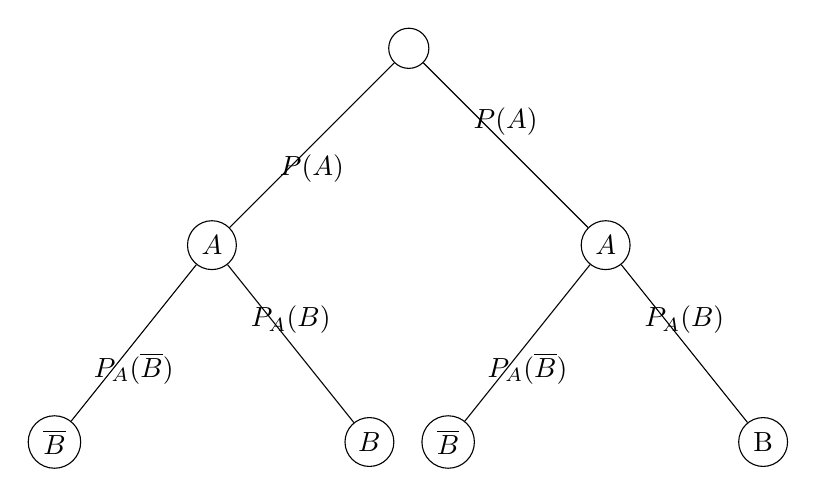
\begin{tikzpicture}[grow=down]
  \node[bag]{}
  child
  {
    node[bag] {$\Bar{A}$} % beschriftet Knoten 2 in erster Ebene mit X
    child
    {
      node[bag] {$\overline{B}$} % beschriftet Knoten 4 in zweiter Ebene mit D
      edge from parent
      node[below]  {$P_{\Bar{A}}(\overline{B})$} % beschriftet Verbindung zu Knoten 4 (Ebene 2) mit p
} child {
      node[bag] {$B$} % beschriftet Knoten 3 in zweiter Ebene mit C
      edge from parent
      node[above]  {$P_{\Bar{A}}(B)$} % beschriftet Verbindung zu Knoten 3 (Ebene 2) mit m
    }
    edge from parent
    node[below]  {$P(\Bar{A})$} % beschriftet Verbindung zu Knoten 2 (Ebene 1) mit f
} child {
    node[bag] {$A$} % beschriftet Knoten 1 in erster Ebene mit A
    child
    {
      node[bag] {$\overline{B}$} % beschriftet Knoten 2 in zweiter Ebene mit B
      edge from parent
      node[below]  {$P_{A}(\overline{B})$} % beschriftet Verbindung zu Knoten 2 (Ebene 2) mit k
} child {
      node[bag] {B} % beschriftet Knoten 1 in zweiter Ebene mit A
      edge from parent
      node[above]  {$P_{A}(B)$} % beschriftet Verbindung zu Knoten 1 (Ebene 2) mit i
    }
    edge from parent
    node[above]  {$P(A)$} % beschriftet Verbindung zu Knoten 1 (Ebene 1) mit w
  };
\end{tikzpicture}
\end{merke*}